% Chapter 2

\chapter{Background Work} % Main chapter title

\label{chapter:background_work} % For referencing the chapter elsewhere, use \ref{Chapter3} 
In this chapter, we will briefly cover machine learning algorithms, then go over published works as they pertain to data stream mining. This will consist of various algorithms, and the current research problems being addressed.

We expect the audience of this thesis to be comfortable in the field of computer science and to have briefly read about or been introduced to machine learning.

\section{Summary}
This chapter presents the fundamentals of machine learning and the various challenges of extracting knowledge from data streams. We introduce classification as a type of machine learning, for which the goal is to extract knowledge, computationally, from labelled data. Algorithms are developed to model the relationship between the data and the class labels. Semi-supervised learning is also a classification task but with the added constraint of learning from a data set that is not entirely labelled. In this thesis, the data we learn from come from data streams, which are voluminous, volatile and velocious. As such, constraints on time and memory usage must be respected, and a mechanism is required to forget "old data" safely.

We cover specific classifiers: baseline classifiers are usually relatively simple and used as a baseline for comparing classifier performance. We also cover the algorithms that we employed in our framework, as well as the state of the art: Naive Bayes, Stochastic Gradient Descent, Hoeffding Trees and Leveraging Bagging.

We define concept drifts as an evolution in the probability distribution of classes and/or attributes. We describe the main types of concept drifts that can occur, regardless of how self-explanatory they are named: abrupt, gradual and recurring. We then review drift detection strategies presented in the literature, including FHDDM/S which we extend in this thesis. Our review shows a gap in research as it pertains to semi-supervised drift detection.

Next, we define ensembles as an amalgamation of a number of classifiers. As all classifiers must output a prediction, ensembles must as well; we present existing techniques to map these multiple outputs to a single one. Having defined ensembles, we review those that were proposed in the literature using two criteria: the processing method and whether or not they were designed to deal with evolving concepts. The processing method distinguishes if instances are analysed online (one-by-one) or in batches. Our review shows a gap in research as it pertains to semi-supervised learning from evolving streams.

\section{Machine Learning Fundamentals}
Within the vast domain of Artificial Intelligence (AI) lies the field of Machine Learning (ML) whose goal is to extract knowledge from data automatically. Given a data set, a model is constructed using a machine learning algorithm to extract knowledge from the attributes in the data. 
Classification is, among others, a method of knowledge extraction called supervised learning. Each item belonging to a given data set must have a nominal class label and a series of pairs of attributes and values. The class label is almost always constrained to a predefined set. A machine learning algorithm is used to model the relationship between the class labels and the attribute/value pairs. Once a model is created, it can predict the class label of any unlabelled data instance (or labelled, as long as the model does not use its value while predicting).

Semi-supervised learning differs (SSL) from traditional supervised learning, by learning from a data set that is not fully labelled, in that not all samples in a data set are labelled.

Initially, classification tasks dealt with static, small, homogeneous data sets. Therefore models created were also static and did not need to be updated, or did not support it. 
Big data, a sub-field of machine learning, arose due to the need to analyse even more voluminous data sets. This required new knowledge extraction techniques to be developed to handle large swaths of data while specifically focusing on keeping computation time and memory usage as low as possible.
More recently, with the advent of the Internet of Things (IoT), more and more data is being generated and streamed online from low-powered (both computationally and due to battery capacity) internet-connected devices. This has developed an interest in the research community to design machine learning algorithms that can learn from data streams, due to the new challenges brought about by this new data medium.

\section{Data Stream Classification}
% \cite{KRAWCZYK2017132}
\subsection{Data Streams}
Krempl et al., in their paper discussing open challenges in data stream mining, use three Vs to describe the main challenges that must be dealt with: volume, volatility and velocity \cite{krempl2014open}. The difficulty with mining data streams is that these three challenges are present simultaneously, while only a subset must typically be dealt with when mining static data sets.

These challenges can be broken down into the following requirements: limiting time taken to process and model incoming data; modelling over a single pass, in an incremental fashion to keep memory bounded and minimal; establishing a mechanism to safely forget "old data" over time, to adapt to changes in the underlying concepts to be modelled \cite{gama2010knowledge, gama2014survey, ghesmoune2016state, KRAWCZYK2017132, krempl2014open, silva2013data, widmer1996learning}.

\subsection{Baseline Classification}
\subsubsection{Majority Class}
This is one of the simplest classifiers. It predicts the class label of a new instance as the currently most frequent class. The majority class algorithm is mostly used as a baseline to determine if another classifier performs better or worse than simply predicting the most frequent class. Due to its simplicity, it satisfies the time requirement stated above by running very quickly, and requires very little maintenance and memory: only an array of counters are needed for each class \cite{bifet2018machine}.

\subsubsection{No-Change}
This is another very simple classifier. It predicts the class of a new instance as the real class of the previously seen instance. This classifier requires even less maintenance than majority class, as it only requires a variable to keep track of the last seen class label \cite{bifet2018machine}.

\subsection{Naive Bayes (NB)}
This algorithm applies the Bayes' theorem with naive feature independence assumptions. Zhang, in his paper discussing the optimality of Naive Bayes, says that it "is one of the most efficient and effective inductive learning algorithms" \cite{zhang2004optimality}. He also proves, that although the feature independence assumption is usually violated in real-world applications, that it can perform optimally if the "dependences distribute evenly in classes, or if the dependences cancel each other out" \cite{zhang2004optimality}.

There are various versions implemented depending on the distribution of the data to be modelled, such as Gaussian NB, Multinomial NB, and Bernouilli NB.

A downside to using NB in an online setting is its inability to learn new concepts unless they are explicitly added to its training set with their new class label.

\subsection{Stochastic Gradient Descent (SGD) Classifier}
Bottou, in his paper discussing tricks for stochastic gradient descent, explains that a loss function measures the cost of predicting $\hat{y}$ when the actual class was $y$, and that the objective is to seek a function, which is parameterized by a weight vector, that minimises that loss.
SGD is a simplification of gradient descent, that estimates the gradient of the empirical risk instead of computing it. The empirical risk measures the training set performance. The estimation of the gradient is based on a randomly selected example from the data at each iteration \cite{bottou2012stochastic}.

The particular version of the SGDClassifier selected, from scikit-learn \cite{scikit-learn}, implements a simple yet very efficient method to learn a logistic regression model under convex loss functions. The advantages, as listed by the authors of this particular implementation, are its efficiency, as previously stated, and its simple implementation. They also list, as its disadvantages, the hyperparameters that the classifier requires and its sensitivity to feature scaling. However, they note that it can "easily scale to problems with more than $10^5$ training examples and more than $10^5$ features" \cite{scikit-learn-sgd}. The authors also cite Bottou and his SGD SVM \cite{bottou2008learning}\footnote{SVMSGD: \url{https://leon.bottou.org/projects/sgd}} and other published works \cite{tsuruoka2009stochastic, shalev2011pegasos} as inspiration for their implementation.

\subsection{Hoeffding Trees / VFDT\label{section:vfdt}}
The main issue with building decision trees in a streaming setting is reusing instances to determine the best splitting criterion for attributes, which is not possible due to the memory requirements for storing all of the data \cite{domingos2000mining}. Domingos and Hulten suggest a Very Fast Decision Tree algorithm for streaming data (VFDT), called Hoeffding Tree in \cite{domingos2000mining}. This tree waits for new instances to arrive instead of reusing data for computing splits. Most interestingly, they find that the resulting tree is almost identical to the one modelled by an offline batch learning algorithm, given enough data to learn from. The algorithm (\ref{alg:vfdt}) is based on the Hoeffding Bound and chooses, as a confidence interval for the entropy at a node, the value:

\begin{equation}
\epsilon=\sqrt{\frac{R^{2} \ln 1 / \delta}{2 n}}
\end{equation}
where R is the range of the random variable, $\delta$ is one minus the desired probability of choosing the correct attribute at any node, and $n$ is the number of examples collected at a node. Lastly in algorithm \ref{alg:vfdt}, $G$ is the heuristic measure to choose test attributes, and could be information gain as seen in C4.5 or some other heuristic \cite{bifet2018machine, domingos2000mining, }

\begin{algorithm}
\caption{Hoeffding Tree\label{alg:vfdt} \cite{bifet2018machine}}
\Fn{HoeffdingTree(Stream, $\delta$)}{
  \KwData{a stream of labelled examples, confidence parameter $\delta$}
    let HT be a tree with a single leaf node\\
  init counts $n_{ijk}$ at root\\
  \For{each example(x,y) in Stream}{
    HTGrow((x,y), HT, $\delta$)\\
  }
}
\setcounter{AlgoLine}{0}
\Fn{HTGrow((x, y), HT, $\delta$)}{
    sort($x, y$) to leaf $l$ using $HT$\\
    update counts $n_{ijk}$ at leaf $l$\\
    \If{examples seen so far at $l$ are not all of the same class}{
        compute $G$ for each attribute\\
      \If{G($\text{best attribute}$) - G($\text{second best}$) > $\sqrt{\frac{R^{2} \ln 1 / \delta}{2 n}}$}{
        split leaf on best attribute\\
          \For{each branch}{
          start new leaf and initialize counts
          }
        }
    }
}
\end{algorithm}

\subsection{Leveraging Bagging\label{section:leveraging-bagging}}
Leveraging Bagging (LB), also called Leverage Bagging, is a classifier ensemble that improves upon the online Oza Bagging algorithm in terms of accuracy, at the cost of higher memory utilisation and an increased execution time \cite{bifet2010leveraging}. In offline bagging, $M$ models are trained, each "with a bootstrap sample of size $N$ created by drawing random samples with replacement from the original training set" \cite{bifet2010leveraging}. Each of the model's training sets should contain the original training set $K$ times.

In online bagging, each sample is assigned a weight according to $Poisson(1)$, instead of sampling with replacement. Bifet, in a study comparing online bagging to online boosting, found that the former was the best method in terms of accuracy \cite{bifet2009new}, but at the cost of a high memory utilisation and execution time, just like LB as we stated above. Bifet also claims that adding more random weights to all instances seems to improve accuracy more than if only adding to the misclassified instances. For this reason, they proposed their online leveraging bagging algorithm with randomisation improvements: increasing the weights of the input samples and adding randomisation to the output of the ensemble via output codes.

The improvements in Leveraging bagging \cite{bifet2010leveraging} therefore come in the form of: first, increasing re-sampling by using a higher parameter for the Poisson distribution, to attribute a wider range of weights to the incoming samples (training samples), thereby increasing the input-space diversity; secondly, through the use of output detection codes: they assign an $n$ bit binary code to each class label, and one of $n$ classifiers are trained on one of those bits in order to correct, to a certain extent, misclassifications. Finally, to deal with concept drift, LB uses one instance of the ADWIN algorithm for each $n$ classifier. When a drift is detected, the classifier associated with the ADWIN detector that has the highest variance in its sliding window is reset (calculated as the average of the numeric values kept in the window). Algorithm \ref{alg:leveraging-bagging} shows the pseudocode for LB.

\begin{algorithm}
\caption{Leveraging Bagging for \text{M} models\label{alg:leveraging-bagging} \cite{bifet2010leveraging}}
Initialise base models $h_{m}$ for all $m \in \{1,2, \ldots, M\}$\\
Compute colouring $\mu_m(y)$\\
\For{\textbf{all} training example(x,y)}{
    \For{$m = {1,2, \ldots, M}$}{
        Set $w = Poisson(\lambda)$\\
        Update $h_m$ with the current example with weight $w$ and class $\mu_m(y)$
    }
    \If{$\text{ADWIN}$ detects change in error of one of the classifiers}{
        Replace classifier with higher error with a new one
    }
    \textbf{anytime output:}
    \Return hypothesis: $h_{fin}(x) = \text{arg max}_{y\in Y}\sum_{t=1}^T I(h_t(x) = \mu_t(y))$
}
\end{algorithm}


\section{Evolving Concepts\label{section:concept_drift}}
In this section, we first define concept drifts and cover the different kinds of drifts that can occur. Strategies presented in the literature are reviewed thereafter.

\subsection{Concept Drift Preliminaries}

We consider two types of streams: those that are stationary and those that are not. The former consists of those where examples are generated randomly from a stationary but unknown probability distribution. The latter consists of streams where the distribution of classes and/or attributes can evolve over time. These evolutions in probability distributions are called concept drifts and occur after periods of stability \cite{gama2010knowledge, KRAWCZYK2017132}. As concept drifts occur, a classifier's model learned from previous data becomes out of date with the current probability distribution and, as a result, its accuracy deteriorates over time. The classifier must then forget its model and start anew.
Ergo, the primary challenge is to detect at which point in time concepts occur. Finally, to detect drifts, an algorithm must "combine robustness to noise with sensitivity to concept change" \cite{gama2010knowledge}.

Real examples of domains with concept drifts include, among others, surveillance systems, telecommunication systems, sensor networks, categorising spam, financial fraud detection and weather predictions. 

Gama formalises concept drift as a change in the joint probability $P(\vec{x}, y)=P(y | \vec{x}) \times P(\vec{x})$ \cite{gama2010knowledge}, that is consistent and persistent.

A consistent concept is defined as a change in the state of the target function over a predetermined threshold between two distinct points in time, whereas a concept is qualified as persistent if measured as consistent over a given time frame. 

This definition, based on cause and effect, allows us to distinguish two types of drift, as well as noise, which table \ref{table:drift-types-def} illustrates. 

\begin{table}[]
\caption{\label{table:drift-types-def}How real drifts differ from virtual drifts, and noise}
\centering
\begin{tabular}{|c|c|c|}
\hline
 & \textbf{Persistent} & \textbf{Consistent} \\ \hhline{===}
\textbf{Real drift} & \checkmark & \checkmark \\ \hline
\textbf{Virtual drift} & $\times$ & \checkmark \\ \hline
\textbf{Noise} & $\times$ & $\times$ \\ \hline
\end{tabular}
\end{table}

In practice, the learning model must be updated regardless of whether a drift is real or virtual.

The most common way to categorise concept drifts, however, is based upon the manner in which changes occur \cite{bifet2018machine}, as figure \ref{fig:concept-drift-types} depicts.

Sudden drifts are characterised by an abrupt change in the distribution generating the data, meaning that a given distribution is suddenly replaced by another distribution instantaneously \cite{tsymbal2004problem}.

Gradual drifts, as their name suggests, present "a slower rate of change". The distribution generating the data is slowly replaced over a longer period of time. In \cite{minku2010impact}, two types of gradual drifts are identified. The first, simply called gradual drifts, samples back and forth from two different distributions by slowly increasing its probability of sampling from the new distribution all the while decreasing from the one being replaced.
The second transitions from two distributions by slowly morphing from one to the other, thereby slowly incorporating incremental changes. During this transition phase, data cannot be attributed to one distribution or another, but rather to a mix of both. These drifts are qualified as incremental.

The last commonly identified type of drift is the recurrent, or re-occurring, drift. Concepts can reappear after some length of time, and may or may not do so in a cyclical fashion meaning that concepts could reappear in a specific order \cite{bifet2018machine, KRAWCZYK2017132, tsymbal2004problem}.


\begin{figure}
  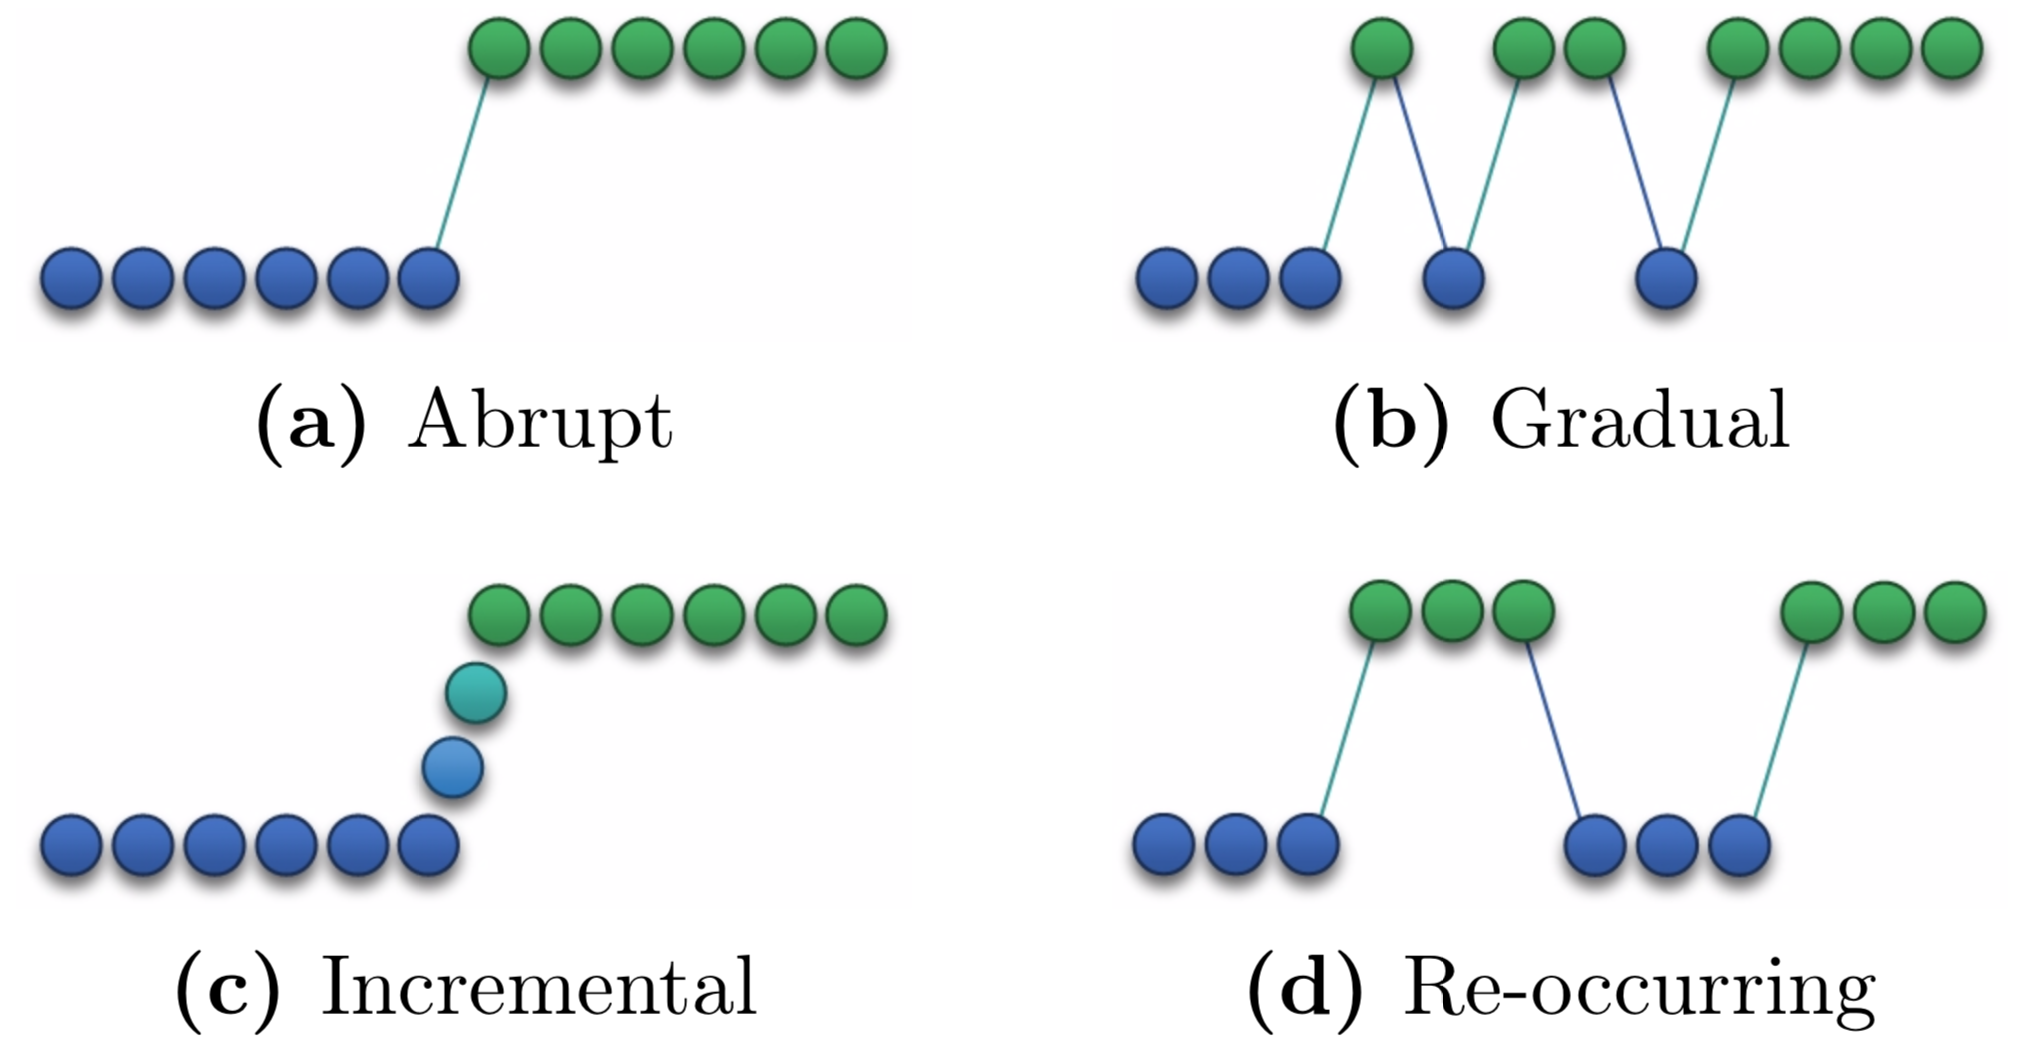
\includegraphics[width=\linewidth]{./images/chapter2/concept-drifts}
\caption{\label{fig:concept-drift-types}Types of drifts \cite{pesaranghader2018reservoirthesis}}
\end{figure}

\subsection{Concept Drift Detection Methods}
Methods to detect drifts do so based on information collected from a classifier's performance or directly from the incoming data. They warn that a drift may be occurring or that one has occurred, which is usually followed by updating, retraining or replacing an old classifier by a new one.

As we previously stated, fully supervised learning of data streams is not very suitable for real-world applications of data stream mining. It logically follows that drift detection methods that rely on a classifier's predictive performance, through the use of class labels, would also not be suitable for real-world applications.

3 metrics are usually considered to measure a drift detector's performance, according to \cite{KRAWCZYK2017132}: the number of correct positive drift detections (real drifts detected), the number of false alarms (no drift present, but detected one erroneously), and the drift detection delay (time between a drift and its actual detection).
As is usually the case, trade-offs are typically made between these three metrics. However, some aggregated measures are proposed in the literature. One such measure is the \textit{acceptable delay length}, proposed by Pesaranghader and Viktor in \cite{pesaranghader2016fast}, that determines if a drift is a true positive by measuring the distance between where a drift is detected and its actual location.

Gama categorises drift detection methods into 4 groups \cite{Gama:2014:SCD:2597757.2523813}, which we will briefly cover in the upcoming paragraphs. These four groups are \textit{Statistical Process Control} methods, \textit{Sequential Analysis} methods, methods that \textit{monitor distributions of 2 different time windows} and \textit{contextual approaches}.

Drift Detection Method (DDM), proposed by Gama in \cite{gama2004learning}, is the most well-known method for the first category. The main idea behind DDM is to monitor the number of errors a classifier makes when predicting. They use the assumption, which they back through statistical theory, that the error-rate should decrease if the distribution generating the incoming data does not change. Consequently, a change in distribution will increase the error rate. They set distinct thresholds for warnings and for drifts. If and when the warning level is reached, incoming instances are to be stored in a special window to be used to retrain the classifier if it ever reaches the drift level. If the drift level is not reached and the error rate drops below the warning level, the window is forgotten, and the drift warning is considered as a false alarm. DDM is not an optimal candidate to be extended for semi-supervised tasks.

Early Drift Detection Method (EEDM) \cite{baena2006early} extends DDM to improve the detection of gradual drifts. Instead of monitoring the \textit{number} of misclassifications, they monitor the \textit{distance between} misclassifications.

Krawczyk, in \cite{KRAWCZYK2017132}, states that sequential probability ratio tests, such as the Wald test, are the basis for detectors that use a \textit{sequential analysis} method.
The Cumulative Sum approach (CUSUM) proposed by Page in \cite{page1954continuous}, computes a weighted sum of the last $k$ examples to detect significant changes in a specified parameter of the probability distribution.

Methods using Hoeffding's (HDDM) and McDiarmid's inequalities were proposed in \cite{frias2015online}. These methods use moving averages and weighted moving averages to detect when a statistic ($p$) deviates "statistically far" from its expected value. The authors use a normal distribution example where the warning would be at 95\% ($p$ differs from $\mu\pm 2\sigma$) and the drift level at 99\% ($p$ differs from $\mu\pm 3\sigma$). The algorithm generalises to any distribution but requires a desired significance level $\alpha_W$ for warnings and $\alpha_D$ for drifts. The authors state that their two methods are independent of classifier choice, have $O(1)$ complexity for time and applicable to scenarios where "labels are harder to obtain". 

Adaptive Windowing (ADWIN2) proposed by Bifet \cite{bifet2007learning} maintains a window of variable size containing bits or real numbers. The size of the window grows when no change is apparent and shrinks when change is apparent. ADWIN requires $O(\log(W)$ update time and memory for a window size of $W$. Change is detected when two distinct sub-windows have a different average. The split index between these two sub-windows is considered as an indication of a drift. ADWIN is a very well known drift detection method, and the best-known method for \textit{monitoring distributions of 2 different time windows}.

As we have previously stated, these drift detection methods rely on timely access to labels which is not a realistic assumption in the real world.  Active-Learning is an approach that has not yet extensively researched.

Unsupervised detection of drifts can rely on, according to \cite{sobolewski2013concept}, non-parametric statistical tests such as the CNF Density Estimation test \cite{dries2009adaptive}, the multivariate version of the Wald–Wolfowitz test \cite{friedman1979multivariate}.
A two-sample Kolmogorov–Smirnov test, a Wilcoxon rank sum test, and a two-sample t-test can also be used to detect drifts in data distribution according to \cite{sheskin2003handbook, sobolewski2013concept}.

\label{paragraph:SAND}SAND is a semi-supervised framework for learning from evolving streams, proposed by Haque in \cite{haque2015sand}. SAND trains $k$-NN estimators (an unsupervised learner, read clustering technique), which regroups $k$ pseudopoints, to detect drifts using each model's confidence. The confidence is averaged from two calculated heuristics for each model: association and purity. Association decreases the further a data point is from a cluster, and purity indicates if a cluster contains mostly one class or a mix of classes. SAND uses a semi-supervised change detector, that consists of storing the confidences in a sliding window, and comparing means from two sub-windows. Drifts are detected when the the mean of the newest confidence values drops below $95\%$ of the mean of older confidence values ($m_a \leq 0.95\times m_b$, where $m_a$ is the mean for the sub-window containing the newest confidence values). The ensemble maintains a good accuracy using a limited amount of labelled data, but none of the experiments specify its execution time.

Our thesis contributes to narrowing the gap in research dealing with semi-supervised drift detection by extending FHDDM to work with unlabelled data, which we cover in the following section.

\subsubsection{FHDDM and FHDDMS\label{section:fhddm/s}}
Pesaranghader, in \parencite{pesaranghader2018reservoirthesis,pesaranghader2018reservoir, pesaranghader2016fast}, proposes two concept drift detection algorithms, with similar characteristics. The first uses a single sliding window, whilst the second uses two sliding windows: one short and the other longer. The sliding window stores a boolean value indicating if the classifier predicted the class properly. His drift detection algorithms keep track of the maximum frequency value seen of correct predictions as well as the current frequency of correct predictions over the sliding window(s), then computes the difference between the maximum and current frequency. Hoeffding's inequality is used to determine the maximum desired difference between an empirical mean and a true mean of \textit{n} random independent variables, without making any assumptions on the distribution of the data. A drift is detected by using Hoeffding's inequality to detect when a significant change occurs between the two frequency measures, meaning that the difference surpasses a given threshold. The author found that FHDDM and FHDDMS were able to detect drifts with smaller delays and greater accuracy when compared to the state-of-the-art. Refer to algorithm \ref{alg:fhddm} for the implementation of FHDDM.

\begin{algorithm}
\caption{Fast Hoeffding Drift Detection Method (FHDDM) \label{alg:fhddm}\cite{pesaranghader2018reservoirthesis,pesaranghader2018reservoir, pesaranghader2016fast}}
\Fn{init(window\_size, delta)}{
    (n, $\delta$) = (window\_size, delta)\;
    $\epsilon_d = \sqrt{\frac{1}{2n}ln\frac{1}{\delta}}$\;
    reset()\;
}

\Fn{reset()}{
    w=[]\;
    $\mu^m=0$\;
}

\Fn{detect(p)}{
    \If{w.size = n}{
        w.tail.drop()\;
    }
    w.push(p)\;
    \eIf{$w.size < n$}{
        return False\;
    }{
        $\mu^t=\frac{w.count(1)}{w.size()}$\;
        \If{$\mu^m < \mu^t$}{
            $\mu^m =\mu^t$\;
        }
        $\Delta\mu = \mu^m - \mu^t$\;
        \eIf{$\Delta\mu \ge \epsilon_d$}{
            reset()\;
            \Return True
        }{
            \Return False
        }
    }
}
\end{algorithm}

%----------------------------------------------------------------------------------------

\section{Ensembles\label{section:ensembles}}
Highlighted in review articles \cite{jain2000statistical, KRAWCZYK2017132, oza2008classifier, polikar2006ensemble, rokach2009taxonomy, wozniak2014survey}, ensembles are considered as one of the most promising research directions nowadays. Ensembles, also known as combined classifiers, multiple classifier systems (MCS), classifier ensembles, classifier fusion, and hybrid classifiers, can also be found reviewed in books \cite{baruque2011fusion, kuncheva2004combining,rokach2010pattern,seni2010ensemble}, and machine-learning handbooks \cite{alpaydin2009introduction, duda2012pattern}.

A supervised ensemble amalgamates any given number of classifiers \cite{KRAWCZYK2017132,opitz1999popular,polikar2006ensemble,rokach2010ensemble}. As an ensemble encapsulates other learning techniques, it needs a strategy to consider each of the classifiers' outputs to make a final prediction. What follows are examples of some such strategies, after which we review supervised ensembles as they pertain to data streams.

\subsection{Ensemble voting strategies\label{section:voting_ensemble}}
When an ensemble predicts a class label for a new instance, each classifier comprised within must predict a class label for the instance and return it to the ensemble. The ensemble then needs to map these multiple, potentially different, predictions to a single output prediction. In order to do so, several functions have been proposed that apply weights to any permutation of the classifiers and/or of their predictions, and then apply a combination rule to these un/weighted values to finally vote on the final output of the ensemble.

Zhou, explains the three following voting techniques in \citep[72-75]{zhou2012ensemble}.

\subsubsection{Majority Voting}
This voting scheme is reportedly the most popular. The method is as simple as it sounds. Each classifier in the ensemble votes for the class label it predicts and the winning class label is the one with at least half the votes. If none of the class labels obtain more than half of the votes, a "rejection option" can be given and no prediction is made by the ensemble. In the case of binary classification, with \textit{n} classifiers, the winning class must have $\lfloor \frac{n}{2} + 1\rfloor$votes. Equation \ref{eq:majority_voting} shows the formula for majority voting. $h_i^j(x) \in [0,1]$ and takes value $1$ if classifier $h_i$ predicts class label $c_j$. $l$ is the number of class labels.

\begin{equation}
    H(x) = 
\begin{cases}
    c_j,& \text{if } \sum^n_{i=1}h^j_i(x) > \frac{1}{2}\sum_{k=1}^{l}\sum_{i=1}^n h_i^k(x)\\
    rejection,              & \text{otherwise}
\end{cases}
\label{eq:majority_voting}
\end{equation} 

\subsubsection{Plurality voting}
This technique is almost identical to majority voting, with the slight difference that it does not require the final class label to obtain more than half of the votes; the final class label obtained the most votes. Ties are broken arbitrarily, and plurality coincides with majority voting in the case of binary classification. Equation \ref{eq:plurality_voting} shows the formula for plurality voting. $h_i^j(x) \in [0,1]$ and takes value $1$ if classifier $h_i$ predicts class label $c_j$.

\begin{equation}
H(x) = c_{arg_j max\sum^n_{i=1}h^j_i(x)}
\label{eq:plurality_voting}
\end{equation}

\subsubsection{Soft voting}
Soft voting differs from plurality voting in that it requires each of the classifiers in the ensemble to output a confidence value (usually in $[0, 1]$) for their prediction for each class value or output the probabilities that an instance belongs to a given class label for all class labels.
In the case of \textit{simple soft voting}, the average probability for each class label is computed over the predictions of all classifiers. The probability of the final class label is given by equation \ref{eq:simple_soft}. Again, $h_i^j(x) \in [0,1]$ and takes value $1$ if classifier $h_i$ predicts class label $c_j$. $L$ is the set of class labels, $l$ here is any label in $L$.

\begin{equation}
H(x)=max( \frac{1}{n}\sum_{i=1}^nh_i^l(x)\ \forall l \in L)
\label{eq:simple_soft}
\end{equation}
There are variations of soft voting where a weight is applied to either each of the classifiers, or to each class, or to each instance. However, Zhou states that in practice, instance weights are typically not used as it may involve a large number of weight coefficients.

\subsection{Review of Ensemble Classifiers \label{section:ensemble_review}}
Krawczyk in his survey reviewing ensemble learning for data streams \cite{KRAWCZYK2017132}, categorises ensemble learning from data streams for supervised classification using two criteria. The first is the data processing method: online, as in one by one, or in chunks. The second one deals with the ensembles' ability to deal with stationary or non-stationary streams, meaning without or with concept drifts. We re-use these two criteria for our review.

As our contributions deal with non-stationary streams, we will focus on reviewing techniques for those.

\subsubsection{Chunk-based ensembles for stationary streams}

Learn$^{++}$ builds incremental neural networks (NN) and uses majority voting to combine their outputs \cite{polikar2001learn++, KRAWCZYK2017132}. However, this technique is unsuitable for large streams, as all NN are retained, memory used continuously increases.

AdaBoost RAN-LTM combines AdaBoost.M1 and Resource Allocating Network with Long-Term Memory. A predetermined number of base classifiers are trained then incrementally updated on new instances \cite{kidera2006incremental, KRAWCZYK2017132}. The forgetting factor is "suppressed" to more efficiently weight voting combinations. Same as for Learn$^{++}$, infinite streams may cause memory usage issues.

Growing Native Correlation Learning (Growing NCL) aims to co-train an ensemble using neural networks. Their algorithm allows for a trade-off between the forgetting rate and the ability to adapt to new data. Experimental results seemed to indicate that fixed size ensembles have a better generalisation ability whereas the growing size may "easily overcome the impact of too strong forgetting" \cite{minku2009negative, KRAWCZYK2017132}

Bagging$^{++}$ was shown to be faster than Learn$^{++}$ and NCL, with comparable results \cite{zhao2010incremental, KRAWCZYK2017132}. It improves upon Learn$^{++}$ through the use of bagging to build new models from incoming data. The ensemble is composed of diverse classifiers selected from a set of four base classifiers.

\subsubsection{Online ensembles for stationary streams}
OzaBag allows the use of bagging in an online setting by replicating newly arriving instances by updating the classifier with $k$ copies of these incoming instances, where $k \sim Poisson(1)$ distribution \cite{oza2005online, KRAWCZYK2017132, }.

Leveraging Bagging (LB), as explained above, adds more randomisation to the input and output of the ensemble, by increasing sampling from $Poisson(1)$ to $Poisson(\lambda)$ where $\lambda$ is a parameter for LB \cite{bifet2010leveraging, KRAWCZYK2017132}.

OzaBoost (also known as Online Boosting) uses a fixed amount of classifiers, which are all trained sequentially on all incoming instances \cite{oza2005online, KRAWCZYK2017132, }. When a classifier misclassifies an instance, the instance's weight is increased to boost its importance to the subsequent classifiers. The first weight is the highest possible value: $\lambda=1$. Then, classifiers are trained $k=\text{Poisson}(\lambda)$ times. Each classifier keeps a count of instances it misclassified ($\epsilon$). If a classifier classifies correctly, then $\lambda = \lambda * \frac{1}{2(1-\epsilon)}$, otherwise $\lambda = \lambda * \frac{1}{2\epsilon}$. The new weight $\lambda$ is then used to train the next classifier.

Ultra Fast Forest of binary Trees (UFFT) makes use of an ensemble of Hoeffding Trees \cite{gama2005learning, KRAWCZYK2017132, }. The split criterion used can only be applied to binary classification problems, but binary decomposition allows for multi-class problems to be handled. Each pair of classes has its own binary tree, which is updated when a new instance has a true class label for one of its two classes.

Ensemble of Online Sequential Extreme Learning Machines (EOS-ELM) \cite{lan2009ensemble, KRAWCZYK2017132} is an improvement on the existing OS-ELM technique. EOS-ELM is composed of initially diverse online neural networks (NN) which are initially trained by using random weights for their single hidden layer. The outputs of the NNs are averaged to obtain the ensemble's output. Incoming data is used to train all NNs in the ensemble sequentially. The authors do not, however, indicate how the classifiers in the ensemble maintain their diversity while learning from the stream.

Other online ensemble techniques for stationary streams include, among others, Ensemble of adaptive-size Hoeffding trees \cite{bifet2009improving}, Online Random Forest \cite{denil2013consistency, saffari2009line}, Online Mondrian Forest \cite{lakshminarayanan2014mondrian}, and Hoeffding Option Trees \cite{gama2010knowledge}.

\subsubsection{Chunk-based ensembles for non-stationary streams}
Many chunk-based ensembles for non-stationary streams use the following approach:
\begin{enumerate}
\item Given a chunk of data $D$ obtained from a stream, evaluate ensemble classifiers $C_j$ on $D$ using evaluation measure $E(C_j)$
\item Train a new classifier $C_i$ on $D$
\item Add $C_i$ to the ensemble if its size permits it, or replace a given classifier in the ensemble
\end{enumerate}

The following algorithms use this approach to varying degrees.

Street and Kim, in \cite{street2001streaming}, propose the well-known Streaming Ensemble Algorithm (SEA). SEA follows the approach stated above, with a precision to be added in step three. If the ensemble size has not been reached, $C_i$ is added to the ensemble. Otherwise, $C_i$, and all other classifiers in the ensemble predict class labels for the next training chunk, and the classifier with the worst quality is replaced with $C_i$. In order to promote diversity and avoid over-fitting, SEA favours classifiers that correctly classifies instances for which the other classifiers in the ensemble are "nearly undecided" \cite{street2001streaming}. Finally, it uses majority voting to map the output predictions of the classifiers for an ensemble prediction. Again, due to the ensemble's reliance on prequential accuracy (and therefore true and timely class labels) to replace the lowest quality classifier, it is not the most suited to deal with late-arriving labels or missing labels. By that same logic, it is neither a prime candidate to be extended to deal with semi-supervised problems. Other potential issues include determining good chunk and ensemble sizes,  that old classifiers can outweigh newer ones thereby "slowing down adaptation to newer concepts" \cite{KRAWCZYK2017132}. SEA does present the following qualities: it uses approximately constant memory, runs quickly, and can adjust quickly to concept drift.

Accuracy Weighting Ensemble (AWE), proposed by Wang et al. in \cite{wang2003mining}, follows the typical approach, with a variation on the replacement strategy. The idea behind AWE is to weight each classifier using a particular variant of the mean square error on the newest chunk using cross-validation. The weight of a classifier is reversely proportional to the estimation of its prediction error. Classifiers are pruned if they predict randomly or worse, or by only keeping a subset of those with the highest weights. This removes classifiers that do not model the current concept well or makes room for newer classifiers to learn new concepts. However, just like previous classifiers, AWE relies on the prequential accuracy for its pruning strategy, and therefore may have difficulty with missing or late-arriving class labels, and requires a different pruning strategy for it to be extended to deal with semi-supervised data. Additionally, the use of cross-validation, for the computation of weights, increases AWE's execution time.

Chu and Zaniolo proposed the Adaptive Boosting ensemble (Aboost) \cite{chu2004fast}, that mixes boosting with a chunk-based input. To detect concept drifts, each time a chunk is received, the ensemble's error is computed. If a concept drift is detected, the entire ensemble is completely reset; otherwise, each instance of the chunk is assigned a weight based on the ensemble's error. This weight is then used to train a new classifier from the weighted chunk, which is added to the ensemble if it is not full; otherwise, it replaces the oldest classifier in the ensemble. Soft voting is used to map the classifier's predictions to a single output for the ensemble. In their experimental evaluation, the authors found that their approach outperformed SEA \cite{street2001streaming} and AWE \cite{wang2003mining} in terms of predictive accuracy. Their technique is also faster, uses less memory and is more adaptive to concept drifts. False flags for concept drifts may cause issues, however, as the entire ensemble is reset. Moreover, as for SEA and AWE, prequential accuracy is relied upon, in this case, to compute weights, making this algorithm susceptible to failure when dealing with missing or late-arriving class labels.

Elwell and Polikar also proposed a chunk-based approach inspired by boosting called \cite{elwell2011incremental} Learn$^{++}$.NSE, that as its name suggests improves upon Learn$^{++}$ to deal with non-stationary environments. The typical approach is again used, with each incoming chunk being used to train a new classifier in the ensemble. Learn$^{++}$.NSE is similar to Adaptive Boosting but differs in that the weights are assigned based on how a classifier predicts as compared to the entire ensemble. A higher weight is assigned if a classifier predicts correctly when the ensemble does not, and a lower weight is assigned in the opposite case. The authors allow their ensemble to learn from new instances while reinforcing existing and still relevant knowledge by giving more importance to recent misclassifications to promote the learning of newer concepts. Furthermore, Learn$^{++}$.NSE uses a weighted majority voting strategy to combine the classifier's predictions, allowing them to assign a minuscule weight to old classifiers representing old concepts. This allows the algorithm to disable a classifier when it does not predict well and to re-enable it when the concept recurs. However, as Learn$^{++}$.NSE allows for an unlimited number of classifiers, the memory used keeps increasing. Again, it presents the same issues for late or missing labels.

\textbf{The following strategies use an alternative approach, that differs from the typical one stated at the start of this section.}

Knowledge-Based Sampling (KBS), a boosting-like method, is proposed by Scholz and Klinkenberg in \cite{scholz2005ensemble}. For each new chunk, depending on which has the best resulting accuracy, a new classifier is trained, or the last trained classifier is updated with the new data. In a boosting-like style, weights are assigned to each instance of a chunk, and weights are also attributed to each classifier based on its predictive accuracy for the new chunk. These weights allow for the pruning of poorly performing classifiers, as well as quickly detecting concept drifts. KBS has been shown to not perform well when dealing with a recurring concept right after an abrupt drift. The authors state that KBS is computationally efficient, and empirically showed that it can "outperform more sophisticated adaptive window and batch selection strategies" \cite{scholz2005ensemble}. However, as all of the other algorithms seen, it relies on prequential accuracy, in this case for its pruning strategy, making it susceptible to failure when dealing with missing or late-arriving class labels.

Batch Weighted Ensemble (BWE) was proposed by Deckert \cite{deckert2011batch} to deal with abrupt and gradual concept drifts. BWE consists of an ensemble with an embedded simple Batch Drift Detector (BDDM). BDDM builds a simple regression model on accumulated accuracy values from each incoming instance, and will only process batches with decreasing trends. BDDM outputs warning or drift flags. When a drift is possible (warning or drift flag), a new classifier is trained on the new batch, and any classifiers that perform worse than a random classifier are discarded. Again, we can see a reliance on prequential accuracy within the ensemble, and therefore it might cause issues when class labels are missing or late-arriving.

Weighted Aging Ensemble (WAE), proposed by Wozniak in \cite{wozniak2013application}, is inspired by AWE \cite{wang2003mining}, and extended with two modifications. The first is that classifiers are weighted based on their prequential accuracy, but also on how much time they spend within the ensemble. The last modification adds classifiers to the ensemble based on their diversity measure.

Other alternative approaches include Accuracy Updated Ensemble (AUE2) by Brzezinksi \cite{brzezinski2014reacting}, and Ensemble Tracking (ET) which deals specifically with recurring concepts by Ramamurthy \cite{ramamurthy2007tracking}.

\subsubsection{Online ensembles for non-stationary streams}

Nishida, in \cite{nishida2007adaptive}, proposes an enhanced version of Adaptive Classifier Ensembles (ACE) that adds a pruning method and improves the voting method. ACE comprises one online classifier, a set of batch classifiers, and a drift detection mechanism. The online classifier is trained on every incoming instance, and a fixed-sized buffer keeps instances that were recently seen. When the buffer is full or a drift is detected, a new batch classifier is created to summarise the data for that time period, the buffer is emptied, and the online classifier is re-initialised. A weighted majority vote is used to compute the output for the ensemble, for which the classifier weights are determined by the predictive accuracy of the classifiers over the last $W$ seen instances. To manage the number of classifiers in the ensemble, the oldest classifier is usually pruned, unless it has good predictive accuracy for the last seen $W$ instances, making use of older data when concepts recur. The size of the buffer kept does not seem to affect ACE's ability to detect abrupt concept drifts, but determining the size of the sliding window containing the $W$ most recently seen instances might prove to be difficult.
Finally, ACE requires timely and correct class labels in order to function correctly, which means it is not a prime candidate to be extended to deal with semi-supervised tasks, or that it be particularly applicable for real-world applications where labels can arrive late, or not at all.

In \cite{bifet2009new}, Bifet proposes Adaptive Windowing (ADWIN) Bagging, which is merely the result of adding an ADWIN drift detector to online bagging (briefly explained in section \ref{section:leveraging-bagging}. ADWIN is responsible for replacing the worst performing classifier in the ensemble with a new classifier when a drift is detected.

Other algorithms that learn using online ensembles over non-stationary streams include \cite{BRZEZINSKI201450, Kolter:2005:UAE:1102351.1102408, Kolter20072755, kuncheva2004classifier, minku2012ddd, stanley2003learning, yoshida2011adaptive}, as well as  the SAND semi-supervised framework \cite{haque2015sand}.

In summary, only one of the articles reviewed that dealt with non-stationary streams did not rely on the prequential accuracy, whether for their weighting scheme, their drift detection, or some other reason, any attempt to extend these algorithms to deal with semi-supervised learning tasks could prove arduous. This constitutes a gap in research which we narrow with our contributions in the next chapter.